2c2
< \label{sec:c5_discussion}
---
> \label{sec:discussion}
5c5
< \label{ssec:c5_comparetoobs}
---
> \label{ssec:comparetoobs}
9c9
< \includegraphics[angle=0,width=0.8\columnwidth]{chapter5_zhu+16/figures/mni.pdf}
---
> \includegraphics[angle=0,width=1.0\columnwidth]{mni.pdf}
11c11
< \label{fig:c5_mni}
---
> \label{fig:mni}
16c16
< We have estimated the range of masses of centrally-simmering sub-\Mch\ WDs that explode, as well as their corresponding \MNi\ yields assuming a pure detonation immediately after simmering.  Putting aside the possibility that extremely strong magnetic fields could affect \vconv, we have also determined that this range does not significantly change when including \dnabconv, rotation or magnetic fields.  It is then interesting to consider in the abstract whether these could reproduce a substantial portion of the SN Ia parameter space, and, to that end, we compare our results to estimates of ejected mass and \Ni\ yields for observed SNe Ia.  In Fig. \ref{fig:c5_mni}, we plot the $\MNi-\Mtot$ relationship for adiabatic and \dnabconv-inclusive WDs, as well as the relationship (also derived using $M(\rho>10^7)$) from the pure detonation of uniform $10^5$ K cold WD for comparison.  Additionally, results from the pure detonation simulations of \cite{sim+10} are plotted to show the accuracy of the $M(\rho>10^7)$ estimate.  Alongside these, we plot the best-fit relationship to the ejected and synthesized \Ni\ masses of $337$ observed ``normal'' \citep{bran+06} SNe Ia from \cite{scalzrs14}, and the estimated \Mtot\ and \MNi\ of $31$ normal SNe Ia from \cite{chil+15}.  \cite{scalzrs14} derives their $\MNi-\Mtot$ relationship from the observed bolometric light curve (using a range of simulated explosion models as priors; \citealt{scalz+14}), and \cite{chil+15} use \cite{scalzrs14}'s method of estimating \Mtot\ while obtaining \MNi\ from the evolution of the $[\textsc{Co\,III}]$ $\lambda5893$ emission complex during the SN Ia nebular phase.
---
> We have estimated the range of masses of centrally-simmering sub-\Mch\ WDs that explode, as well as their corresponding \MNi\ yields assuming a pure detonation immediately after simmering.  Putting aside the possibility that extremely strong magnetic fields could affect \vconv, we have also determined that this range does not significantly change when including \dnabconv, rotation or magnetic fields.  It is then interesting to consider in the abstract whether these could reproduce a substantial portion of the SN Ia parameter space, and, to that end, we compare our results to estimates of ejected mass and \Ni\ yields for observed SNe Ia.  In Fig. \ref{fig:mni}, we plot the $\MNi-\Mtot$ relationship for adiabatic and \dnabconv-inclusive WDs, as well as the relationship (also derived using $M(\rho>10^7)$) from the pure detonation of uniform $10^5$ K cold WD for comparison.  Additionally, results from the pure detonation simulations of \cite{sim+10} are plotted to show the accuracy of the $M(\rho>10^7)$ estimate.  Alongside these, we plot the best-fit relationship to the ejected and synthesized \Ni\ masses of $337$ observed ``normal'' \citep{bran+06} SNe Ia from \cite{scalzrs14}, and the estimated \Mtot\ and \MNi\ of $31$ normal SNe Ia from \cite{chil+15}.  \cite{scalzrs14} derives their $\MNi-\Mtot$ relationship from the observed bolometric light curve (using a range of simulated explosion models as priors; \citealt{scalz+14}), and \cite{chil+15} use \cite{scalzrs14}'s method of estimating \Mtot\ while obtaining \MNi\ from the evolution of the $[\textsc{Co\,III}]$ $\lambda5893$ emission complex during the SN Ia nebular phase.
21c21
< As expected from previous analysis, the $\MNi-\Mtot$ relationship changes little between the adiabatic and \dnabconv-inclusive WDs, being separated by a $\Mtot\lesssim0.01\,\Msun$ for any given \MNi.  While not plotted, we also found that this is true for WDs rotating at $50$\% of critical, and those with $\sim10^{11}\,\mrm{G}$ magnetic fields.  The previously-noted steep dependence of \MNi\ on \Mtot\ near \Mcrit\ is clear as well: a linear fit around $\Mtot = 1.15\,\Msun$ gives $d\MNi/d\Mtot \approx 10$ (for both curves), making it difficult to accurately estimate a minimum \MNi.  This also leads to a fine-tuning problem: to produce \MNi\ between $\sim0.3-0.6\,\Msun$ -- typical \MNi\ yields in \cite{scalzrs14} and \cite{chil+15} -- requires \Mtot\ to lie in a narrow range between $\sim 1.13 - 1.17\,\Msun$.  It is not obvious why a progenitor channel would favor this mass range, though we note the distribution of field CO WD masses is very narrowly peaked (at $0.65\,\Msun$; eg. \citealt{tremb09, klei+13}), possibly indicating that merging CO WD binaries masses fall within a narrow range.
---
> As expected from previous analysis, the $\MNi-\Mtot$ relationship changes little between the adiabatic and \dnabconv-inclusive WDs, being separated by a $\Mtot\lesssim0.01\,\Msun$ for any given \MNi.  While not plotted, we also found that this is true for WDs rotating at $50$\% of critical, and those with $\sim10^{11}\,\mrm{G}$ magnetic fields.  The previously-noted steep dependence of \MNi\ on \Mtot\ near \Mcrit\ is clear as well: a linear fit around $\Mtot = 1.15\,\Msun$ gives $d\MNi/d\Mtot \approx 10$ (for both curves), making it difficult to accurately estimate a minimum \MNi.  This also leads to a fine-tuning problem: to produce \MNi\ between $\sim0.3-0.6\,\Msun$ -- typical \MNi\ yields in \cite{scalzrs14} and \cite{chil+15} -- requires \Mtot\ to lie in a narrow range between $\sim 1.13 - 1.17\,\Msun$.  It is not obvious why a progenitor channel would favour this mass range, though we note the distribution of field CO WD masses is very narrowly peaked (at $0.65\,\Msun$; eg. \citealt{tremb09, klei+13}), possibly indicating that merging CO WD binaries masses fall within a narrow range.
27c27
< Nevertheless, the $\MNi-\Mtot$ relationship from pure detonations of centrally simmering CO WDs does not resemble the observed ones.  \cite{chil+15}'s values could be systematically offset by $\sim 0.1\,\Msun$ in \Mtot\ and $\sim 0.2\,\Msun$ in \MNi, but these apply to the points as a whole, and we also do not reproduce the shape of \cite{chil+15}'s distribution.  This issue is not unique to our work - \cite{scalzrs14} and \cite{chil+15} plot theoretical $\MNi-\Mtot$ curves for a wide range of proposed SN Ia progenitor classes, ranging from sub-\Mch\ WDs undergoing a double-detonation (equivalent to the Cold WD line in Fig. \ref{fig:c5_mni}) to \Mch\ pure deflagrations, and find no individual class able to reproduce the entire observed $\MNi-\Mtot$ parameter space.  If their results indeed reflect the true \Mtot-\Ni\ relationship of SNe Ia, either multiple progenitor channels are necessary, or a novel understanding of progenitors must arise.
---
> Nevertheless, the $\MNi-\Mtot$ relationship from pure detonations of centrally simmering CO WDs does not resemble the observed ones.  \cite{chil+15}'s values could be systematically offset by $\sim 0.1\,\Msun$ in \Mtot\ and $\sim 0.2\,\Msun$ in \MNi, but these apply to the points as a whole, and we also do not reproduce the shape of \cite{chil+15}'s distribution.  This issue is not unique to our work - \cite{scalzrs14} and \cite{chil+15} plot theoretical $\MNi-\Mtot$ curves for a wide range of proposed SN Ia progenitor classes, ranging from sub-\Mch\ WDs undergoing a double-detonation (equivalent to the Cold WD line in Fig. \ref{fig:mni}) to \Mch\ pure deflagrations, and find no individual class able to reproduce the entire observed $\MNi-\Mtot$ parameter space.  If their results indeed reflect the true \Mtot-\Ni\ relationship of SNe Ia, either multiple progenitor channels are necessary, or a novel understanding of progenitors must arise.
32c32
< \label{ssec:c5_implications}
---
> \label{ssec:implications}
34c34
< Regardless of whether simmering sub-\Mch\ WDs can reproduce observations, what implications do our results have on double-degenerate CO WD mergers as SN Ia progenitors, in particular the channel of \citeal{vkercj10} involving sub-\Mch\ merger remnants that ignite central nuclear fusion following their viscous evolution?  A direct mapping of post-viscous remnants onto our hydrostatic simmering WDs is not possible since their structures are quite complex, and in general their temperature profiles are substantially shallower than the convective ones used in our models.  Moreover, much of their mass exists as a hot, tenuous envelope that surrounds and exerts little pressure support on their dense, degeneracy-supported ``cores''.  As a rough estimate, we can consider the evolution of these cores as separate from their envelopes (the transition region between the two might resemble the hot atmospheres in Sec. \ref{sssec:c5_runaway_ad_hot}, and thus not affect the core's evolution).
---
> Regardless of whether simmering sub-\Mch\ WDs can reproduce observations, what implications do our results have on double-degenerate CO WD mergers as SN Ia progenitors, in particular the channel of \citeal{vkercj10} involving sub-\Mch\ merger remnants that ignite central nuclear fusion following their viscous evolution?  A direct mapping of post-viscous remnants onto our hydrostatic simmering WDs is not possible since their structures are quite complex, and in general their temperature profiles are substantially shallower than the convective ones used in our models.  Moreover, much of their mass exists as a hot, tenuous envelope that surrounds and exerts little pressure support on their dense, degeneracy-supported ``cores''.  As a rough estimate, we can consider the evolution of these cores as separate from their envelopes (the transition region between the two might resemble the hot atmospheres in Sec. \ref{sssec:runaway_ad_hot}, and thus not affect the core's evolution).
36c36
< Regardless of their initial conditions, the simmering tracks of a remnant core cannot simultaneously increase in temperature and density, since this would require part of their structure to cool (Sec. \ref{ssec:c5_numericalmodels}).  They also cannot exist, for longer than a few convective timescales, to the right of the rising portion of the simmering track of the same mass in Fig. \ref{fig:c5_runaway_rhot}, i.e. the portion of the track between the start of simmering and either the \citeal{wooswk04} point or the point of maximum temperature.  Doing so would mean its temperature gradient has become steeper than the convective one, and convective energy transport will rapidly lower the gradient back to the convective one (like for stars to the right of the Hayashi track).  As a consequence of these two restrictions, \Mcrit\ will increase for those WDs with shallow temperature profiles.  With this in mind, meaningful conclusions can be made by examining the central densities and core masses \Mc\ of post-viscous remnants.
---
> Regardless of their initial conditions, the simmering tracks of a remnant core cannot simultaneously increase in temperature and density, since this would require part of their structure to cool (Sec. \ref{ssec:numericalmodels}).  They also cannot exist, for longer than a few convective timescales, to the right of the rising portion of the simmering track of the same mass in Fig. \ref{fig:runaway_rhot}, i.e. the portion of the track between the start of simmering and either the \citeal{wooswk04} point or the point of maximum temperature.  Doing so would mean its temperature gradient has become steeper than the convective one, and convective energy transport will rapidly lower the gradient back to the convective one (like for stars to the right of the Hayashi track).  As a consequence of these two restrictions, \Mcrit\ will increase for those WDs with shallow temperature profiles.  With this in mind, meaningful conclusions can be made by examining the central densities and core masses \Mc\ of post-viscous remnants.
40c40
< To our knowledge, the sole published viscous evolution simulation of a sub-\Mch\ double CO WD merger remnant is that of \cite{ji+13}.  They find, by the end of their simulation, the central density and temperature of their $0.6 - 0.6\,\Msun$ remnant are $\sim5\times10^6\,\gcc$ and $\sim9\times10^8\,\mrm{K}$, respectively, well above the $\taucc = \taunu$ line.  Indeed, its $\taucc \sim 1\,\mrm{yr}$, much smaller than the $\gtrsim 10^4\,\mrm{yr}$ thermal contraction timescale \citep{shen+12}, so the remnant will begin to simmer.  The mass of the remnant that is within $r = 1.5\times10^9\,\mrm{cm}$ (the approximate outer boundary of the dense core in \citealt{ji+13} Fig. 1) is $\sim1.07\,\Msun$ (Suoqing Ji and Robert Fisher private communication, 2016), $\sim0.06\,\Msun$ lower than \Mcrit.  The remnant's central density is a factor of $\sim4$ lower than that for the $\sim1.05\,\Msun$ simmering track at the same temperature and a factor of $\sim6$ lower than that for the \Mcrit\ simmering track.\footnote{The remnant in \citep{ji+13} has not lost all of its rotational support by the end of their simulation, so its central density will continue to increase early in its simmering phase.  As less than a third of its initial angular momentum remains, however, it is unlikely to increase by a factor of $\sim4$.}  The most likely fate of this system is therefore expansion and possibly stable nuclear burning.  The relatively small difference between \Mc\ and \Mcrit\ suggests a merger remnant $\sim0.1\,\Msun$ more massive might possess a core mass in excess of \Mcrit.  That core's central density, though, may still be too low for simmering to end in an explosion.
---
> To our knowledge, the sole published viscous evolution simulation of a sub-\Mch\ double CO WD merger remnant is that of \cite{ji+13}.  They find, by the end of their simulation, the central density and temperature of their $0.6 - 0.6\,\Msun$ remnant are $\sim5\times10^6\,\gcc$ and $\sim9\times10^8\,\mrm{K}$, respectively, well above the $\taucc = \taunu$ line.  Indeed, its $\taucc \sim 1\,\mrm{yr}$, much smaller than the $\gtrsim 10^4\,\mrm{yr}$ thermal contraction timescale \citep{shen+12}, so the remnant will begin to simmer.  The mass of the remnant that is within $r = 1.5\times10^9\,\mrm{cm}$ (the approximate outer boundary of the dense core in \citealt{ji+13} Fig. 1) is $\sim1.07\,\Msun$ (Suoqing Ji and Robert Fisher private communication), $\sim0.06\,\Msun$ lower than \Mcrit.  The remnant's central density is a factor of $\sim4$ lower than that for the $\sim1.05\,\Msun$ simmering track at the same temperature and a factor of $\sim6$ lower than that for the \Mcrit\ simmering track.\footnote{The remnant in \citep{ji+13} has not lost all of its rotational support by the end of their simulation, so its central density will continue to increase early in its simmering phase.  As less than a third of its initial angular momentum remains, however, it is unlikely to increase by a factor of $\sim4$.}  The most likely fate of this system is therefore expansion and possibly stable nuclear burning.  The relatively small difference between \Mc\ and \Mcrit\ suggests a merger remnant $\sim0.1\,\Msun$ more massive might possess a core mass in excess of \Mcrit.  That core's central density, though, may still be too low for simmering to end in an explosion.
46c46
< For a broader parameter space of post-viscous remnants, we turn to the simple estimate of viscous evolution outcomes made in Sec. \ref{sec:c2_postmerger}.  While it tends to overestimate compression, particularly for remnants from similar-mass mergers, when compared to \citeauthor{schw+12} (and follow-up work in \citealt{rask+14}) and \cite{ji+13}, it nevertheless gives a rough estimate of the post-viscous remnant parameter space.  Taking our estimate at face value, we find that only those remnants from mergers with primary WD masses above $\sim0.8\,\Msun$ have $\rhoc \gtrsim 3\times10^7\,\gcc$, which also suggests that only remnants with total masses above \Mch\ are likely to achieve dynamical burning following viscous spin-down.  Note that the most massive of these may have instead already exploded from extreme temperatures during their mergers (for primary WD masses $\gtrsim0.9\,\Msun$; \citealt{pakm+10,pakm+11}), or due to hydrodynamic instabilities immediately afterward (for primaries $\gtrsim1\,\Msun$; \citealt{kash+15}).
---
> For a broader parameter space of post-viscous remnants, we turn to the simple estimate of viscous evolution outcomes made in \citeal{zhu+13} Sec. 6.1.  While it tends to overestimate compression, particularly for remnants from similar-mass mergers, when compared to \citeauthor{schw+12} (and follow-up work in \citealt{rask+14}) and \cite{ji+13}, it nevertheless gives a rough estimate of the post-viscous remnant parameter space.  Taking our estimate at face value, we find that only those remnants from mergers with primary WD masses above $\sim0.8\,\Msun$ have $\rhoc \gtrsim 3\times10^7\,\gcc$, which also suggests that only remnants with total masses above \Mch\ are likely to achieve dynamical burning following viscous spin-down.  Note that the most massive of these may have instead already exploded from extreme temperatures during their mergers (for primary WD masses $\gtrsim0.9\,\Msun$; \citealt{pakm+10,pakm+11}), or due to hydrodynamic instabilities immediately afterward (for primaries $\gtrsim1\,\Msun$; \citealt{kash+15}).
61c61
< \label{ssec:c5_magaccuracy}
---
> \label{ssec:magaccuracy}
63c63
< We found in Sec. \ref{ssec:c5_rotmag} that $\lesssim10^{11}\,\mrm{G}$ magnetic fields negligibly affect simmering, while $\gtrsim10^{12}\,\mrm{G}$ ones could dramatically affect \vconv, but there are reasons to be cautious about these results, particularly in the strong field limit.
---
> We found in Sec. \ref{ssec:rotmag} that $\lesssim10^{11}\,\mrm{G}$ magnetic fields negligibly affect simmering, while $\gtrsim10^{12}\,\mrm{G}$ ones could dramatically affect \vconv, but there are reasons to be cautious about these results, particularly in the strong field limit.
67c67
< First, \citeal{stev79} does not include convective dynamo processes that amplify the magnetic field.  The vigorous convection zone found toward the end of simmering is an ideal environment for such processes -- analogous to the highly magnetized central convection zones of A and B main sequence stars (eg. \citealt{brunbt05, feat+09, augubt16}).  Amplification saturates when $\EBEconv \sim 1$, i.e. when, 
---
> First, \citeal{stev79} does not include convective dynamo processes that amplify the magnetic field.  The vigorous convection zone found toward the end of simmering is an ideal environment for such processes -- analagous to the highly magnetized central convection zones of A and B main sequence stars (eg. \citealt{brunbt05, feat+09, augubt16}).  Amplification saturates when $\EBEconv \sim 1$, i.e. when, 
73c73
< \noindent For WDs at the end of simmering, $B_\mrm{eq} \sim 3\times10^{11}-1\times10^{12}\,\mrm{G}$.  These values match or exceed any magnetic fields generated by the merger or viscous evolution (though having fields in place at the start of simmering may increase the saturation field strength by up to another order of magnitude; \citealt{feat+09}), rendering even the low-field calculations uncertain.  Additionally, the turbulent nature of the dynamo will generate a highly tangled magnetic field that varies significantly over short length scales, unlike the large-scale fields assumed in this work; Eqn. \ref{eq:c5_dnabmag_est_work} would then suggest a much larger \dnabmag\ \citep{chabgb07}.
---
> \noindent For WDs at the end of simmering, $B_\mrm{eq} \sim 3\times10^{11}-1\times10^{12}\,\mrm{G}$.  These values match or exceed any magnetic fields generated by the merger or viscous evolution (though having fields in place at the start of simmering may increase the saturation field strength by up to another order of magnitude; \citealt{feat+09}), rendering even the low-field calculations uncertain.  Additionally, the turbulent nature of the dynamo will generate a highly tangled magnetic field that varies significantly over short length scales, unlike the large-scale fields assumed in this work; Eqn. \ref{eq:dnabmag_est_work} would then suggest a much larger \dnabmag\ \citep{chabgb07}.
75c75
< Second, studies of nonlinear magnetoconvection (eg. \citealt{procw82}) indicate that in steady state, magnetic fields are concentrated into high-flux bundles where the convective flow is truncated, surrounded by regions where convection continues uninhibited.  The amount of convective suppression depends on the volume fraction the bundles occupy.  When the ratio \EBEconv\ between magnetic and convective kinetic energy densities becomes higher than unity, the bundles merge and convection is effectively suppressed.  This physical picture (which is fundamentally multi-dimensional) shares little resemblance with \citeal{stev79} (Henk Spruit private communication, 2016), and no magnetic equivalent of \cite{barkdl14}'s examination of rotating convection has been conducted to see if \citeal{stev79} at least phenomenologically captures it.
---
> Second, studies of nonlinear magnetoconvection (eg. \citealt{procw82}) indicate that in steady state, magnetic fields are concentrated into high-flux bundles where the convective flow is truncated, surrounded by regions where convection continues uninhibited.  The amount of convective suppression depends on the volume fraction the bundles occupy.  When the ratio \EBEconv\ between magnetic and convective kinetic energy densities becomes higher than unity, the bundles merge and convection is effectively suppressed.  This physical picture (which is fundamentally multi-dimensional) shares little resemblance with \citeal{stev79} (Henk Spruit private communication), and no magnetic equivalent of \cite{barkdl14}'s examination of rotating convection has been conducted to see if \citeal{stev79} at least phenomenologically captures it.
81c81
< Our model's inability to accurately follow magnetoconvection and include dynamo processes therefore constitutes the greatest uncertainty of this work.  While we have estimated that including rotation without magnetic fields is important only because it modifies the hydrostatic balance of the WD, rotation coupled with both convection and magnetic fields may additionally lead to unexpected emergent behavior.  The multidimensional nature of magnetoconvection may also alter the end of simmering criterion -- for example, if burning material is trapped within a flux bundle, it may locally run away and lead to dynamical burning even if convection is unhindered elsewhere in the WD.  We thus stress the need for more detailed investigation into WD magnetoconvection, potentially utilizing MHD convective simulations, in the future.
---
> Our model's inability to accurately follow magnetoconvection and include dynamo processes therefore constitutes the greatest uncertainty of this work.  While we have estimated that including rotation without magnetic fields is important only because it modifies the hydrostatic balance of the WD, rotation coupled with both convection and magnetic fields may additionally lead to unexpected emergent behaviour.  The multidimensional nature of magnetoconvection may also alter the end of simmering criterion -- for example, if burning material is trapped within a flux bundle, it may locally run away and lead to dynamical burning even if convection is unhindered elsewhere in the WD.  We thus stress the need for more detailed investigation into WD magnetoconvection, potentially utilizing MHD convective simulations, in the future.
